\documentclass{scrartcl}

\usepackage[utf8x]{inputenc}
\usepackage{graphicx}
\usepackage{booktabs}
\usepackage{titling}
\usepackage{xcolor}
\usepackage{amsmath}
\usepackage{amsfonts}
\usepackage[a4paper, margin=.9in]{geometry}
% 

\setlength{\droptitle}{-7.5em}

\title{Causal Inference for Policy Evaluation\\
\Large{Assignment 2}}
\author{Marco Gortan, Felix Schulz, Benjamin Weggelaar}
\date{\today}

\newcommand{\marco}[1]{\textcolor{red}{#1}}
\newcommand{\felix}[1]{\textcolor{cyan}{#1}}
\newcommand{\benji}[1]{\textcolor{green}{#1}}

\begin{document}

\maketitle

\section*{Question 1}

\begin{table}[!h]
\centering
\caption{\label{tab:tab:np_atet}Internet access and employment: Non-parametric bootstrap estimates of ATET}
\centering
\begin{tabular}[t]{rrrr}
\toprule
ATET & SD & Lower Bound & Upper Bound\\
\midrule
0.0082699 & 0.0033568 & 0.0016905 & 0.0148492\\
\bottomrule
\end{tabular}
\end{table}


\paragraph*{(b)}

\textbf{i.} The parametrically estimated effects are identical until at least the fourth decimal position. This is to be expected since both are calculating the same two differences: In the parametric model, \textit{Submarines} captures the trend before and after treatment across all groups, while \textit{Connected} captures the difference between treatment and control group shared across periods. In the nonparametric approach we are explicitly calculating these two differences (first $\tilde{Y}_i = \bar{Y}_{i,1} - \bar{Y}_{i,0}$ and then $\tilde{Y}_1 - \tilde{Y}_0$).
\textbf{ii.} Standard errors differ by a small amount. Asymptotically and if the OLS assumptions on error variance hold, both should be identical.


\begin{table}
\caption{Parametric ATET estimates}
\begin{center}
\begin{tabular}{l c c c}
\hline
 & No fixed effects, no clustered SE & No fixed effects, clustered SE & Fixed effects, clustered SE \\
\hline
Intercept               & $0.719 \; (0.001)^{***}$  & $0.719 \; (0.004)^{***}$  &                         \\
Connected               & $0.048 \; (0.003)^{***}$  & $0.048 \; (0.010)^{***}$  &                         \\
Submarines              & $-0.040 \; (0.002)^{***}$ & $-0.040 \; (0.004)^{***}$ &                         \\
Treatment               & $0.008 \; (0.005)$        & $0.008 \; (0.010)$        & $0.022 \; (0.008)^{**}$ \\
\hline
Num. obs.               & $280641$                  & $280641$                  & $280641$                \\
R$^2$ (full model)      & $0.003$                   & $0.003$                   & $0.138$                 \\
R$^2$ (proj model)      & $$                        & $$                        & $0.000$                 \\
Adj. R$^2$ (full model) & $0.003$                   & $0.003$                   & $0.128$                 \\
Adj. R$^2$ (proj model) & $$                        & $$                        & $0.000$                 \\
Num. groups: time       & $$                        & $$                        & $10$                    \\
Num. groups: location   & $$                        & $$                        & $3169$                  \\
\hline
\multicolumn{4}{l}{\scriptsize{$^{***}p<0.001$; $^{**}p<0.01$; $^{*}p<0.05$}}
\end{tabular}
\label{table:coefficients}
\end{center}
\end{table}


% Look into whether there is a paper that claims this

\paragraph*{(c)} These standard errors are substantially larger than the previous estimates.

\paragraph*{(d)} The point estimate is larger than the non-parametric estimate. The fixed effect approach used here uses the within estimator, focusing on within-location variation, additionally accounting for temporal fixed effects. The remaining variation after demeaning significantly differs and thereby also the coefficients. We expect to obtain different coefficients as, in the original specification, we were not taking into effect unobservable differences among locations (that differ in their initial employment situation) and the common effects that certain year-quarters have on the employment level.  

% effect is larger
% should we expect them to be different?

\section*{Question 2}

\paragraph*{(a)}
% Do you think that is a good idea to control for the dummy for being skilled? Explain.
Yes, it is a good idea, because we expect skill to be correlated with both treatment and the outcome. Note that if \textit{Skilled} was a time-invariant characteristic of each location, than it would not be needed to be included, as its effect would be absorbed by location fixed effect. 

\paragraph*{(b)}
% Compare the result with the estimate from point 1.d. and comment
The estimate is lower compared to point 1d, suggesting that skilled people go to live close to newly connected grids. Indeed, we see that the coefficient of \textit{Skilled} is positive and significant, absorbing part of the effect that was present in point 1d.

\section*{Question 3}

\paragraph*{(a)}
% Provide a possible explanation for the trends you observe.
The first thing we observe is that \textit{Connected} locations have a higher share of educated people. One potential explanation is that living closer to the grid already allowed faster internet, attracting higher educated people. Moreover, we see that not connected locations are witnessing downward trend in the share of highly educated, possibly due to the fact educated people might migrate more to other areas / countries with job opportunities more similar to their education. Finally, we observe an increase of highly educated people in connected areas after fast internet arrived, possibly due to an increase in education opportunities.  

\begin{figure}[h!]
    \centering
    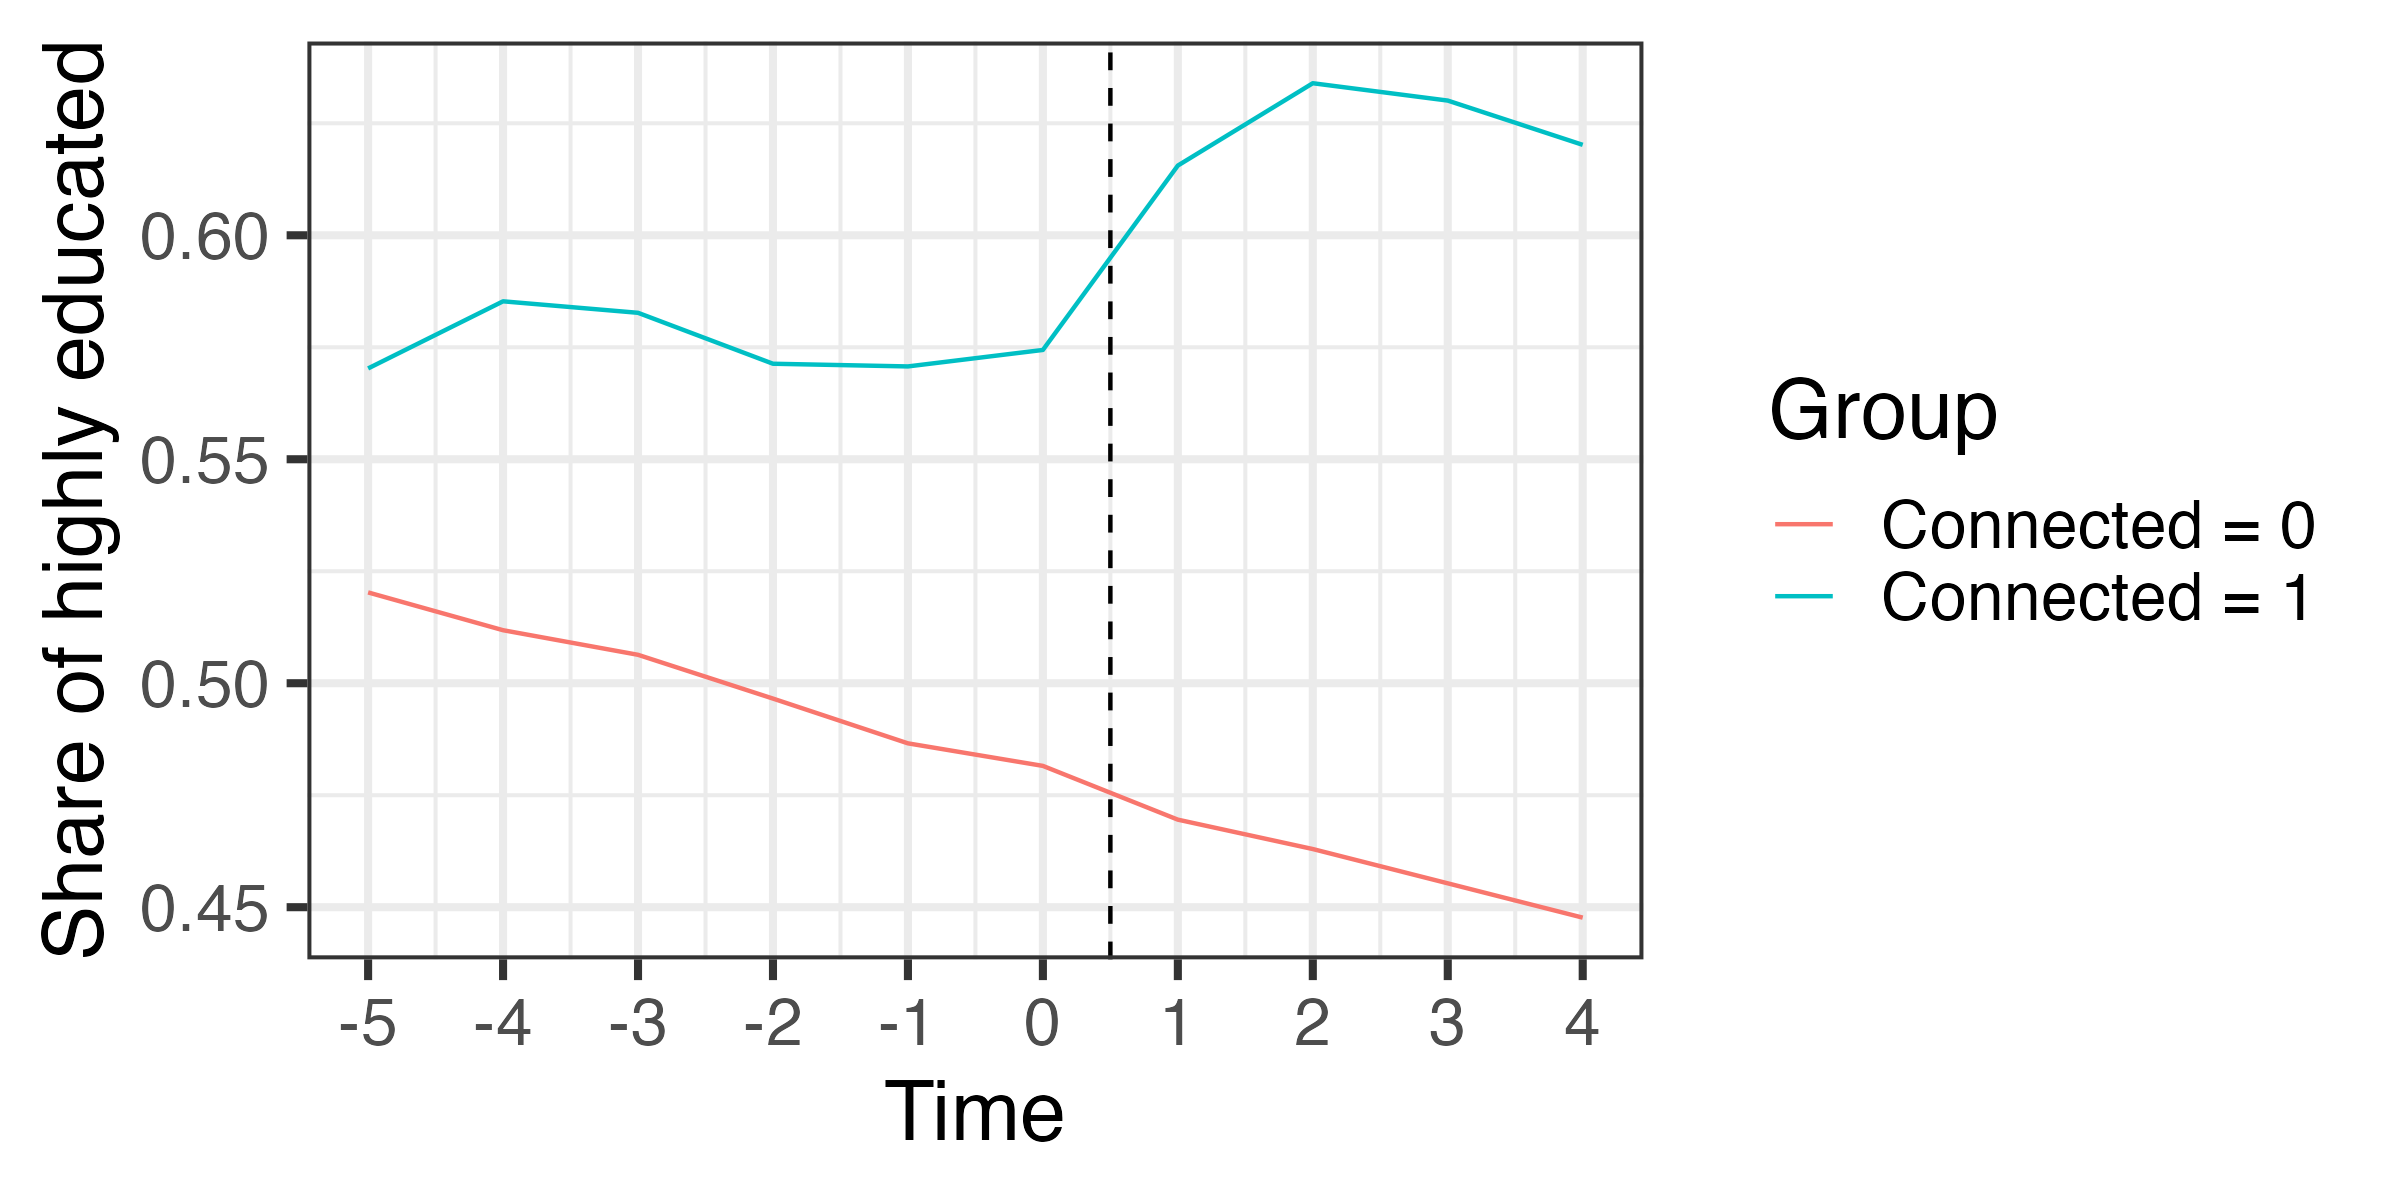
\includegraphics[width=0.75\linewidth]{output/figures/2_common_trends.png}
    \caption{Common trends for education}
    \label{fig:commontrends}
\end{figure}

\paragraph*{(b)}

\begin{figure}[h!]
    \centering
    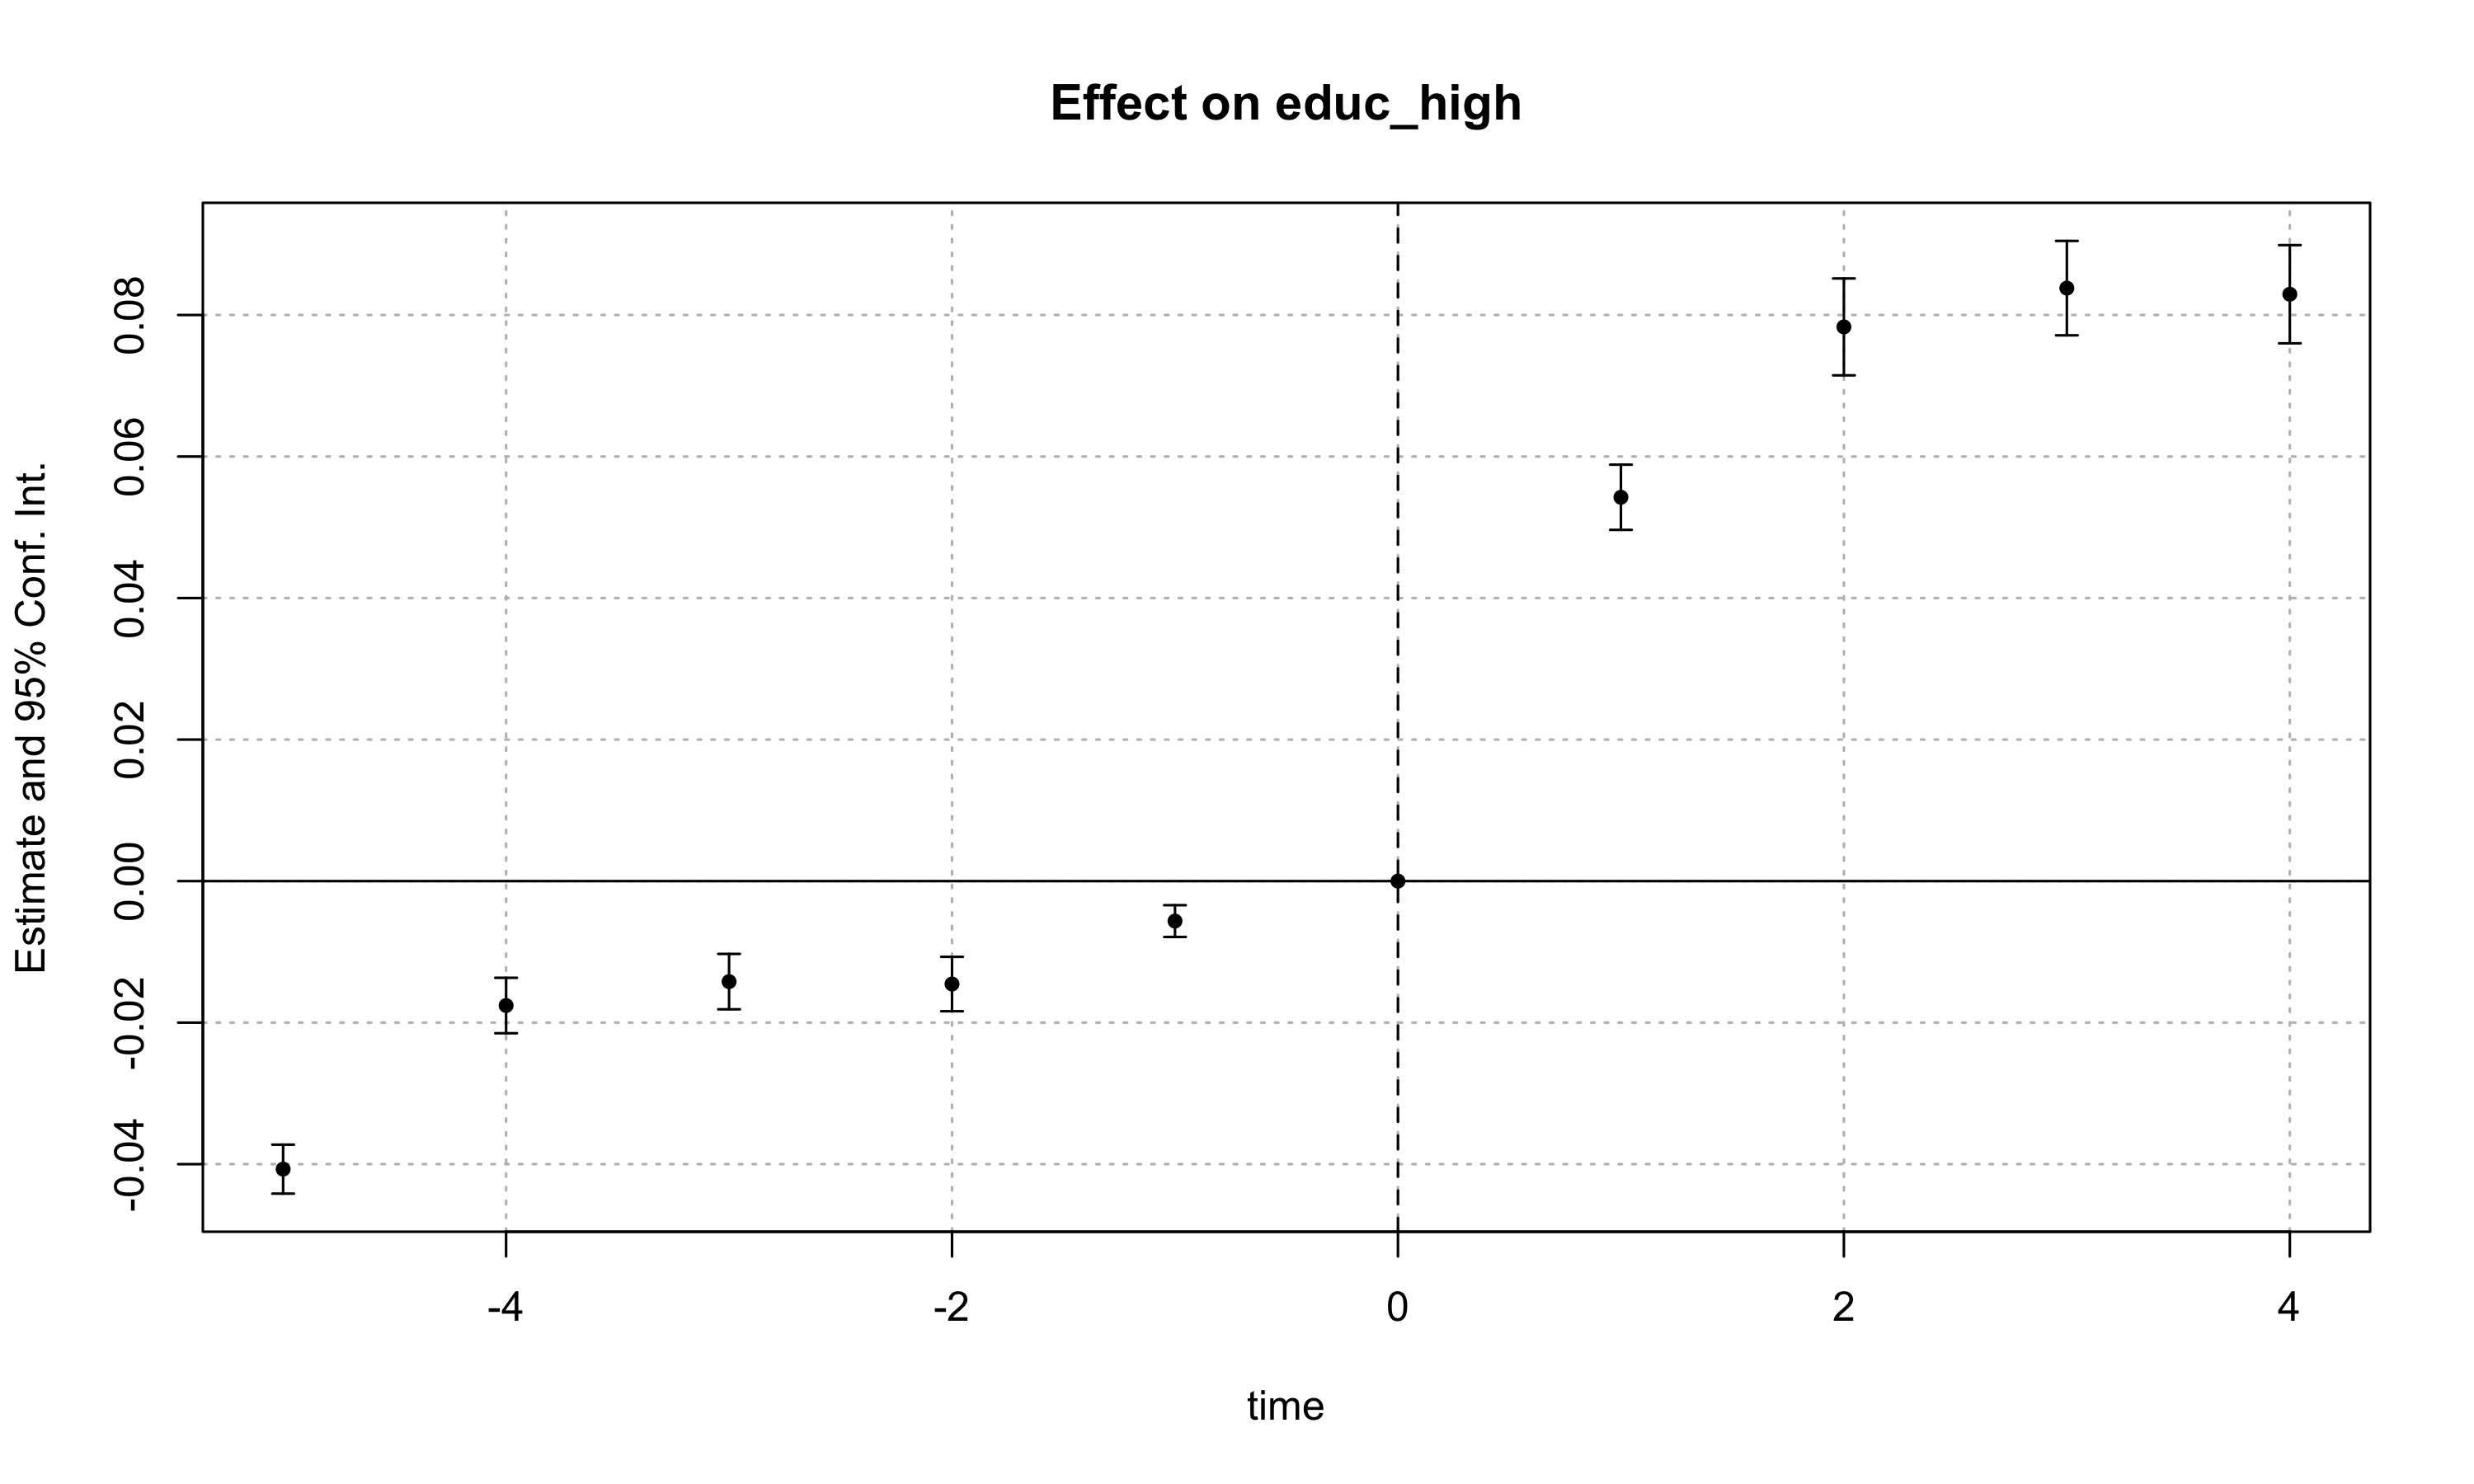
\includegraphics[width=0.75\linewidth]{output/figures/2_event_study.png}
    \caption{Event study: education}
    \label{fig:eventstudy}
\end{figure}

% Conduct an event study for the outcome educ high and report the results in a plot. Based on the results from this and the last question, is it reasonable to use a DiD strategy for this outcome variable?

No. Already prior to treatment, education in those locations further away from the internet network showed a vastly different trend than those that would be treated later. Therefore we cannot confidently assume parallel trends after treatment. 

\paragraph*{(c)}

% Given the common trend plot above, if you were to estimate the effect of fast internet using a DiD strategy, can we say whether our estimate would be up-ward or downward biased? 

Our estimate on employment would be upward biased because we observe a (i) downward trend in not connected locations and a (ii) a flat trend in connected locations before fast internet arrived.

\section*{Question 4}
% Is the result similar to that in point 1.c?

\paragraph*{(a)} Yes, they are similar to the analytical standard errors with unit-clustering from 1(c).

\begin{table}[!h]
\centering
\caption{\label{tab:tab:np_atet_clustered}Internet access and employment: Non-parametric bootstrap estimates of ATET, Cluster-robust SEs}
\centering
\begin{tabular}[t]{rrrr}
\toprule
atet & sd & lower\_bound & upper\_bound\\
\midrule
0.0082699 & 0.0093528 & -0.0100616 & 0.0266013\\
\bottomrule
\end{tabular}
\end{table}


\section*{Question 5}

\paragraph*{(a)}

% Why can’t we just regress female labour supply on the number of children to estimate a causal effect?

In this particular example, regressing female labor supply on the number of children would lead to endogeneity, caused by the omitted variable bias. This is because deciding on the number of children may be influenced by unobserved family factors such as their preferences for leisure over work, access to child care, or family support. This violates the exogeneity or zero conditional mean error assumption that OLS relies on for unbiased and consistent estimates.

\paragraph*{(b)}

% The IV strategy of the authors only identifies a very specific average treatment effect. What is that? Be precise and context-specific

The estimated treatment effect is a local average treatment effect (LATE), because the authors identify the effect of having a third child on labor supply, for those parents whose decision of having a third child is affected by the sex composition of the first two children (same sex). Therefore, the estimated effect is specific to that group. \\
This subset of parents would be called compliers, while parents that would have three children regardless would be considered always-takers, and parents that would have two children regardless of their sex, would be never-takers. The estimated causal effect is specific to the compliers group.

\paragraph*{(c)}

% Consider columns 1 and 2 in Table 7, which presents OLS and IV estimates, respectively. Provide an explanation for why the OLS estimate are lower than the IV ones (i.e. OLS over-estimates the negative effect).

The OLS estimate over-estimates the causal effect because it is unable to isolate the effect of an additional child on labor supply, since it doesn't take into account unobserved factors such as preferences for leisure over work, access to child care, or family support. The result is an estimated effect that combines the true effect of an additional child, plus the effect of these unobserved factors. \\
Using IV terminology, The OLS estimate would also include the always-takers, i.e., parents that would have three children regardless, and these parents may be fundamentally different in their unobserved factors compared to the compliers, which are parents that would only have additional children when the first two are of the same sex.

\end{document}
